\documentclass[1p]{elsarticle_modified}
%\bibliographystyle{elsarticle-num}

%\usepackage[colorlinks]{hyperref}
%\usepackage{abbrmath_seonhwa} %\Abb, \Ascr, \Acal ,\Abf, \Afrak
\usepackage{amsfonts}
\usepackage{amssymb}
\usepackage{amsmath}
\usepackage{amsthm}
\usepackage{scalefnt}
\usepackage{amsbsy}
\usepackage{kotex}
\usepackage{caption}
\usepackage{subfig}
\usepackage{color}
\usepackage{graphicx}
\usepackage{xcolor} %% white, black, red, green, blue, cyan, magenta, yellow
\usepackage{float}
\usepackage{setspace}
\usepackage{hyperref}

\usepackage{tikz}
\usetikzlibrary{arrows}

\usepackage{multirow}
\usepackage{array} % fixed length table
\usepackage{hhline}

%%%%%%%%%%%%%%%%%%%%%
\makeatletter
\renewcommand*\env@matrix[1][\arraystretch]{%
	\edef\arraystretch{#1}%
	\hskip -\arraycolsep
	\let\@ifnextchar\new@ifnextchar
	\array{*\c@MaxMatrixCols c}}
\makeatother %https://tex.stackexchange.com/questions/14071/how-can-i-increase-the-line-spacing-in-a-matrix
%%%%%%%%%%%%%%%

\usepackage[normalem]{ulem}

\newcommand{\msout}[1]{\ifmmode\text{\sout{\ensuremath{#1}}}\else\sout{#1}\fi}
%SOURCE: \msout is \stkout macro in https://tex.stackexchange.com/questions/20609/strikeout-in-math-mode

\newcommand{\cancel}[1]{
	\ifmmode
	{\color{red}\msout{#1}}
	\else
	{\color{red}\sout{#1}}
	\fi
}

\newcommand{\add}[1]{
	{\color{blue}\uwave{#1}}
}

\newcommand{\replace}[2]{
	\ifmmode
	{\color{red}\msout{#1}}{\color{blue}\uwave{#2}}
	\else
	{\color{red}\sout{#1}}{\color{blue}\uwave{#2}}
	\fi
}

\newcommand{\Sol}{\mathcal{S}} %segment
\newcommand{\D}{D} %diagram
\newcommand{\A}{\mathcal{A}} %arc


%%%%%%%%%%%%%%%%%%%%%%%%%%%%%5 test

\def\sl{\operatorname{\textup{SL}}(2,\Cbb)}
\def\psl{\operatorname{\textup{PSL}}(2,\Cbb)}
\def\quan{\mkern 1mu \triangleright \mkern 1mu}

\theoremstyle{definition}
\newtheorem{thm}{Theorem}[section]
\newtheorem{prop}[thm]{Proposition}
\newtheorem{lem}[thm]{Lemma}
\newtheorem{ques}[thm]{Question}
\newtheorem{cor}[thm]{Corollary}
\newtheorem{defn}[thm]{Definition}
\newtheorem{exam}[thm]{Example}
\newtheorem{rmk}[thm]{Remark}
\newtheorem{alg}[thm]{Algorithm}

\newcommand{\I}{\sqrt{-1}}
\begin{document}

%\begin{frontmatter}
%
%\title{Boundary parabolic representations of knots up to 8 crossings}
%
%%% Group authors per affiliation:
%\author{Yunhi Cho} 
%\address{Department of Mathematics, University of Seoul, Seoul, Korea}
%\ead{yhcho@uos.ac.kr}
%
%
%\author{Seonhwa Kim} %\fnref{s_kim}}
%\address{Center for Geometry and Physics, Institute for Basic Science, Pohang, 37673, Korea}
%\ead{ryeona17@ibs.re.kr}
%
%\author{Hyuk Kim}
%\address{Department of Mathematical Sciences, Seoul National University, Seoul 08826, Korea}
%\ead{hyukkim@snu.ac.kr}
%
%\author{Seokbeom Yoon}
%\address{Department of Mathematical Sciences, Seoul National University, Seoul, 08826,  Korea}
%\ead{sbyoon15@snu.ac.kr}
%
%\begin{abstract}
%We find all boundary parabolic representation of knots up to 8 crossings.
%
%\end{abstract}
%\begin{keyword}
%    \MSC[2010] 57M25 
%\end{keyword}
%
%\end{frontmatter}

%\linenumbers
%\tableofcontents
%
\newcommand\colored[1]{\textcolor{white}{\rule[-0.35ex]{0.8em}{1.4ex}}\kern-0.8em\color{red} #1}%
%\newcommand\colored[1]{\textcolor{white}{ #1}\kern-2.17ex	\textcolor{white}{ #1}\kern-1.81ex	\textcolor{white}{ #1}\kern-2.15ex\color{red}#1	}

{\Large $\underline{12a_{0757}~(K12a_{0757})}$}

\setlength{\tabcolsep}{10pt}
\renewcommand{\arraystretch}{1.6}
\vspace{1cm}\begin{tabular}{m{100pt}>{\centering\arraybackslash}m{274pt}}
\multirow{5}{120pt}{
	\centering
	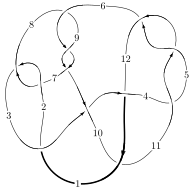
\includegraphics[width=112pt]{../../../GIT/diagram.site/Diagrams/png/1558_12a_0757.png}\\
\ \ \ A knot diagram\footnotemark}&
\allowdisplaybreaks
\textbf{Linearized knot diagam} \\
\cline{2-2}
 &
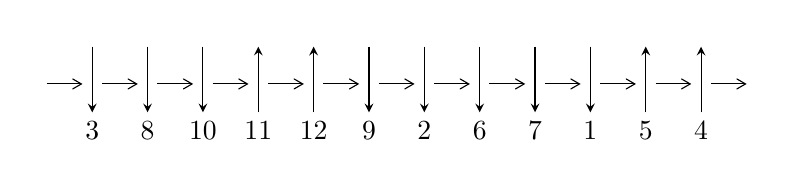
\begin{tikzpicture}[x=20pt, y=17pt]
	% nodes
	\node (C0) at (0, 0) {};
	\node (C1) at (1, 0) {};
	\node (C1U) at (1, +1) {};
	\node (C1D) at (1, -1) {3};

	\node (C2) at (2, 0) {};
	\node (C2U) at (2, +1) {};
	\node (C2D) at (2, -1) {8};

	\node (C3) at (3, 0) {};
	\node (C3U) at (3, +1) {};
	\node (C3D) at (3, -1) {10};

	\node (C4) at (4, 0) {};
	\node (C4U) at (4, +1) {};
	\node (C4D) at (4, -1) {11};

	\node (C5) at (5, 0) {};
	\node (C5U) at (5, +1) {};
	\node (C5D) at (5, -1) {12};

	\node (C6) at (6, 0) {};
	\node (C6U) at (6, +1) {};
	\node (C6D) at (6, -1) {9};

	\node (C7) at (7, 0) {};
	\node (C7U) at (7, +1) {};
	\node (C7D) at (7, -1) {2};

	\node (C8) at (8, 0) {};
	\node (C8U) at (8, +1) {};
	\node (C8D) at (8, -1) {6};

	\node (C9) at (9, 0) {};
	\node (C9U) at (9, +1) {};
	\node (C9D) at (9, -1) {7};

	\node (C10) at (10, 0) {};
	\node (C10U) at (10, +1) {};
	\node (C10D) at (10, -1) {1};

	\node (C11) at (11, 0) {};
	\node (C11U) at (11, +1) {};
	\node (C11D) at (11, -1) {5};

	\node (C12) at (12, 0) {};
	\node (C12U) at (12, +1) {};
	\node (C12D) at (12, -1) {4};
	\node (C13) at (13, 0) {};

	% arrows
	\draw[->,>={angle 60}]
	(C0) edge (C1) (C1) edge (C2) (C2) edge (C3) (C3) edge (C4) (C4) edge (C5) (C5) edge (C6) (C6) edge (C7) (C7) edge (C8) (C8) edge (C9) (C9) edge (C10) (C10) edge (C11) (C11) edge (C12) (C12) edge (C13) ;	\draw[->,>=stealth]
	(C1U) edge (C1D) (C2U) edge (C2D) (C3U) edge (C3D) (C4D) edge (C4U) (C5D) edge (C5U) (C6U) edge (C6D) (C7U) edge (C7D) (C8U) edge (C8D) (C9U) edge (C9D) (C10U) edge (C10D) (C11D) edge (C11U) (C12D) edge (C12U) ;
	\end{tikzpicture} \\
\hhline{~~} \\& 
\textbf{Solving Sequence} \\ \cline{2-2} 
 &
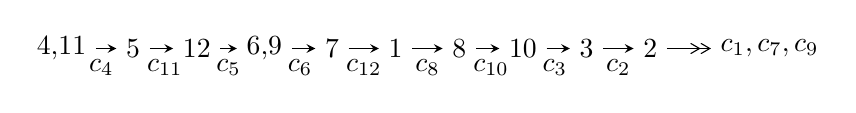
\begin{tikzpicture}[x=23pt, y=7pt]
	% node
	\node (A0) at (-1/8, 0) {4,11};
	\node (A1) at (1, 0) {5};
	\node (A2) at (2, 0) {12};
	\node (A3) at (49/16, 0) {6,9};
	\node (A4) at (33/8, 0) {7};
	\node (A5) at (41/8, 0) {1};
	\node (A6) at (49/8, 0) {8};
	\node (A7) at (57/8, 0) {10};
	\node (A8) at (65/8, 0) {3};
	\node (A9) at (73/8, 0) {2};
	\node (C1) at (1/2, -1) {$c_{4}$};
	\node (C2) at (3/2, -1) {$c_{11}$};
	\node (C3) at (5/2, -1) {$c_{5}$};
	\node (C4) at (29/8, -1) {$c_{6}$};
	\node (C5) at (37/8, -1) {$c_{12}$};
	\node (C6) at (45/8, -1) {$c_{8}$};
	\node (C7) at (53/8, -1) {$c_{10}$};
	\node (C8) at (61/8, -1) {$c_{3}$};
	\node (C9) at (69/8, -1) {$c_{2}$};
	\node (A10) at (11, 0) {$c_{1},c_{7},c_{9}$};

	% edge
	\draw[->,>=stealth]	
	(A0) edge (A1) (A1) edge (A2) (A2) edge (A3) (A3) edge (A4) (A4) edge (A5) (A5) edge (A6) (A6) edge (A7) (A7) edge (A8) (A8) edge (A9) ;
	\draw[->>,>={angle 60}]	
	(A9) edge (A10);
\end{tikzpicture} \\ 

\end{tabular} \\

\footnotetext{
The image of knot diagram is generated by the software ``\textbf{Draw programme}" developed by Andrew Bartholomew(\url{http://www.layer8.co.uk/maths/draw/index.htm\#Running-draw}), where we modified some parts for our purpose(\url{https://github.com/CATsTAILs/LinksPainter}).
}\phantom \\ \newline 
\centering \textbf{Ideals for irreducible components\footnotemark of $X_{\text{par}}$} 
 
\begin{align*}
I^u_{1}&=\langle 
u^{85}-38 u^{83}+\cdots+b+1,\;u^{84}- u^{83}+\cdots+a+2,\;u^{86}-2 u^{85}+\cdots-4 u-1\rangle \\
I^u_{2}&=\langle 
b,\;- u^4- u^3+u^2+a+u,\;u^5+u^4-2 u^3- u^2+u-1\rangle \\
\\
\end{align*}
\raggedright * 2 irreducible components of $\dim_{\mathbb{C}}=0$, with total 91 representations.\\
\footnotetext{All coefficients of polynomials are rational numbers. But the coefficients are sometimes approximated in decimal forms when there is not enough margin.}
\newpage
\renewcommand{\arraystretch}{1}
\centering \section*{I. $I^u_{1}= \langle u^{85}-38 u^{83}+\cdots+b+1,\;u^{84}- u^{83}+\cdots+a+2,\;u^{86}-2 u^{85}+\cdots-4 u-1 \rangle$}
\flushleft \textbf{(i) Arc colorings}\\
\begin{tabular}{m{7pt} m{180pt} m{7pt} m{180pt} }
\flushright $a_{4}=$&$\begin{pmatrix}1\\0\end{pmatrix}$ \\
\flushright $a_{11}=$&$\begin{pmatrix}0\\u\end{pmatrix}$ \\
\flushright $a_{5}=$&$\begin{pmatrix}1\\- u^2\end{pmatrix}$ \\
\flushright $a_{12}=$&$\begin{pmatrix}u\\- u^3+u\end{pmatrix}$ \\
\flushright $a_{6}=$&$\begin{pmatrix}- u^2+1\\u^4-2 u^2\end{pmatrix}$ \\
\flushright $a_{9}=$&$\begin{pmatrix}- u^{84}+u^{83}+\cdots-3 u-2\\- u^{85}+38 u^{83}+\cdots-3 u-1\end{pmatrix}$ \\
\flushright $a_{7}=$&$\begin{pmatrix}u^{84}- u^{83}+\cdots+u^2+2\\- u^{51}+23 u^{49}+\cdots-2 u^2- u\end{pmatrix}$ \\
\flushright $a_{1}=$&$\begin{pmatrix}- u^3+2 u\\- u^3+u\end{pmatrix}$ \\
\flushright $a_{8}=$&$\begin{pmatrix}- u^{84}+u^{83}+\cdots-5 u-3\\-2 u^{85}+76 u^{83}+\cdots-8 u-2\end{pmatrix}$ \\
\flushright $a_{10}=$&$\begin{pmatrix}u^7-4 u^5+4 u^3\\u^7-3 u^5+2 u^3+u\end{pmatrix}$ \\
\flushright $a_{3}=$&$\begin{pmatrix}- u^{14}+7 u^{12}-18 u^{10}+19 u^8-4 u^6-4 u^4+1\\- u^{14}+6 u^{12}-13 u^{10}+10 u^8+2 u^6-4 u^4- u^2\end{pmatrix}$ \\
\flushright $a_{2}=$&$\begin{pmatrix}- u^{25}+12 u^{23}+\cdots-2 u^3+u\\- u^{25}+11 u^{23}+\cdots+5 u^5+u\end{pmatrix}$\\&\end{tabular}
\flushleft \textbf{(ii) Obstruction class $= -1$}\\~\\
\flushleft \textbf{(iii) Cusp Shapes $= -6 u^{85}+4 u^{84}+\cdots-25 u-14$}\\~\\
\newpage\renewcommand{\arraystretch}{1}
\flushleft \textbf{(iv) u-Polynomials at the component}\newline \\
\begin{tabular}{m{50pt}|m{274pt}}
Crossings & \hspace{64pt}u-Polynomials at each crossing \\
\hline $$\begin{aligned}c_{1}\end{aligned}$$&$\begin{aligned}
&u^{86}+33 u^{85}+\cdots+7680 u+1024
\end{aligned}$\\
\hline $$\begin{aligned}c_{2},c_{7}\end{aligned}$$&$\begin{aligned}
&u^{86}+u^{85}+\cdots+64 u+32
\end{aligned}$\\
\hline $$\begin{aligned}c_{3}\end{aligned}$$&$\begin{aligned}
&u^{86}+2 u^{85}+\cdots-3956 u-757
\end{aligned}$\\
\hline $$\begin{aligned}c_{4},c_{5},c_{11}\end{aligned}$$&$\begin{aligned}
&u^{86}-2 u^{85}+\cdots-4 u-1
\end{aligned}$\\
\hline $$\begin{aligned}c_{6},c_{8},c_{9}\end{aligned}$$&$\begin{aligned}
&u^{86}-6 u^{85}+\cdots+6 u-1
\end{aligned}$\\
\hline $$\begin{aligned}c_{10}\end{aligned}$$&$\begin{aligned}
&u^{86}-18 u^{85}+\cdots-31954 u+1153
\end{aligned}$\\
\hline $$\begin{aligned}c_{12}\end{aligned}$$&$\begin{aligned}
&u^{86}+6 u^{85}+\cdots+48 u+5
\end{aligned}$\\
\hline
\end{tabular}\\~\\
\newpage\renewcommand{\arraystretch}{1}
\flushleft \textbf{(v) Riley Polynomials at the component}\newline \\
\begin{tabular}{m{50pt}|m{274pt}}
Crossings & \hspace{64pt}Riley Polynomials at each crossing \\
\hline $$\begin{aligned}c_{1}\end{aligned}$$&$\begin{aligned}
&y^{86}+31 y^{85}+\cdots-28966912 y+1048576
\end{aligned}$\\
\hline $$\begin{aligned}c_{2},c_{7}\end{aligned}$$&$\begin{aligned}
&y^{86}-33 y^{85}+\cdots-7680 y+1024
\end{aligned}$\\
\hline $$\begin{aligned}c_{3}\end{aligned}$$&$\begin{aligned}
&y^{86}-6 y^{85}+\cdots-13406188 y+573049
\end{aligned}$\\
\hline $$\begin{aligned}c_{4},c_{5},c_{11}\end{aligned}$$&$\begin{aligned}
&y^{86}-78 y^{85}+\cdots-8 y+1
\end{aligned}$\\
\hline $$\begin{aligned}c_{6},c_{8},c_{9}\end{aligned}$$&$\begin{aligned}
&y^{86}-74 y^{85}+\cdots-18 y+1
\end{aligned}$\\
\hline $$\begin{aligned}c_{10}\end{aligned}$$&$\begin{aligned}
&y^{86}+30 y^{85}+\cdots-95840184 y+1329409
\end{aligned}$\\
\hline $$\begin{aligned}c_{12}\end{aligned}$$&$\begin{aligned}
&y^{86}-6 y^{85}+\cdots-324 y+25
\end{aligned}$\\
\hline
\end{tabular}\\~\\
\newpage\flushleft \textbf{(vi) Complex Volumes and Cusp Shapes}
$$\begin{array}{c|c|c}  
\text{Solutions to }I^u_{1}& \I (\text{vol} + \sqrt{-1}CS) & \text{Cusp shape}\\
 \hline 
\begin{aligned}
u &= -1.091010 + 0.090090 I \\
a &= -0.956544 + 0.537574 I \\
b &= -0.493444 - 0.302436 I\end{aligned}
 & -0.575276 - 0.519687 I & \phantom{-0.000000 } 0 \\ \hline\begin{aligned}
u &= -1.091010 - 0.090090 I \\
a &= -0.956544 - 0.537574 I \\
b &= -0.493444 + 0.302436 I\end{aligned}
 & -0.575276 + 0.519687 I & \phantom{-0.000000 } 0 \\ \hline\begin{aligned}
u &= \phantom{-}1.094950 + 0.151003 I \\
a &= -1.23286 - 0.93748 I \\
b &= -2.64637 - 1.01452 I\end{aligned}
 & -1.57274 + 2.87671 I & \phantom{-0.000000 } 0 \\ \hline\begin{aligned}
u &= \phantom{-}1.094950 - 0.151003 I \\
a &= -1.23286 + 0.93748 I \\
b &= -2.64637 + 1.01452 I\end{aligned}
 & -1.57274 - 2.87671 I & \phantom{-0.000000 } 0 \\ \hline\begin{aligned}
u &= -0.855622 + 0.201501 I \\
a &= \phantom{-}0.719578 - 0.625350 I \\
b &= \phantom{-}2.47832 - 0.23964 I\end{aligned}
 & -8.00416 + 0.05306 I & -10.12496 + 0.65924 I \\ \hline\begin{aligned}
u &= -0.855622 - 0.201501 I \\
a &= \phantom{-}0.719578 + 0.625350 I \\
b &= \phantom{-}2.47832 + 0.23964 I\end{aligned}
 & -8.00416 - 0.05306 I & -10.12496 - 0.65924 I \\ \hline\begin{aligned}
u &= -1.110730 + 0.237283 I \\
a &= \phantom{-}0.953610 - 0.941499 I \\
b &= \phantom{-}2.19457 - 0.80602 I\end{aligned}
 & -4.00442 - 8.63773 I & \phantom{-0.000000 } 0 \\ \hline\begin{aligned}
u &= -1.110730 - 0.237283 I \\
a &= \phantom{-}0.953610 + 0.941499 I \\
b &= \phantom{-}2.19457 + 0.80602 I\end{aligned}
 & -4.00442 + 8.63773 I & \phantom{-0.000000 } 0 \\ \hline\begin{aligned}
u &= -1.121590 + 0.183537 I \\
a &= -0.313878 - 0.392217 I \\
b &= -0.511985 + 0.231496 I\end{aligned}
 & \phantom{-}1.26195 - 4.79212 I & \phantom{-0.000000 } 0 \\ \hline\begin{aligned}
u &= -1.121590 - 0.183537 I \\
a &= -0.313878 + 0.392217 I \\
b &= -0.511985 - 0.231496 I\end{aligned}
 & \phantom{-}1.26195 + 4.79212 I & \phantom{-0.000000 } 0\\
 \hline 
 \end{array}$$\newpage$$\begin{array}{c|c|c}  
\text{Solutions to }I^u_{1}& \I (\text{vol} + \sqrt{-1}CS) & \text{Cusp shape}\\
 \hline 
\begin{aligned}
u &= \phantom{-}1.204880 + 0.082857 I \\
a &= \phantom{-}0.377988 - 0.117095 I \\
b &= \phantom{-}0.653932 + 0.222912 I\end{aligned}
 & \phantom{-}2.68827 + 0.56424 I & \phantom{-0.000000 } 0 \\ \hline\begin{aligned}
u &= \phantom{-}1.204880 - 0.082857 I \\
a &= \phantom{-}0.377988 + 0.117095 I \\
b &= \phantom{-}0.653932 - 0.222912 I\end{aligned}
 & \phantom{-}2.68827 - 0.56424 I & \phantom{-0.000000 } 0 \\ \hline\begin{aligned}
u &= -0.304717 + 0.718199 I \\
a &= -3.02965 + 2.28213 I \\
b &= -2.85170 - 0.19298 I\end{aligned}
 & -4.47476 - 12.25720 I & -8.16453 + 9.33775 I \\ \hline\begin{aligned}
u &= -0.304717 - 0.718199 I \\
a &= -3.02965 - 2.28213 I \\
b &= -2.85170 + 0.19298 I\end{aligned}
 & -4.47476 + 12.25720 I & -8.16453 - 9.33775 I \\ \hline\begin{aligned}
u &= -0.644967 + 0.406996 I \\
a &= \phantom{-}0.81693 - 1.29819 I \\
b &= \phantom{-}2.40453 - 0.03748 I\end{aligned}
 & -3.18368 + 8.27801 I & -5.74606 - 4.15811 I \\ \hline\begin{aligned}
u &= -0.644967 - 0.406996 I \\
a &= \phantom{-}0.81693 + 1.29819 I \\
b &= \phantom{-}2.40453 + 0.03748 I\end{aligned}
 & -3.18368 - 8.27801 I & -5.74606 + 4.15811 I \\ \hline\begin{aligned}
u &= -0.302147 + 0.698378 I \\
a &= \phantom{-}1.69695 - 0.39760 I \\
b &= \phantom{-}1.200740 + 0.251003 I\end{aligned}
 & \phantom{-}0.59979 - 7.98524 I & -4.28596 + 8.59628 I \\ \hline\begin{aligned}
u &= -0.302147 - 0.698378 I \\
a &= \phantom{-}1.69695 + 0.39760 I \\
b &= \phantom{-}1.200740 - 0.251003 I\end{aligned}
 & \phantom{-}0.59979 + 7.98524 I & -4.28596 - 8.59628 I \\ \hline\begin{aligned}
u &= \phantom{-}0.290094 + 0.690020 I \\
a &= \phantom{-}3.62527 + 2.53458 I \\
b &= \phantom{-}3.21306 - 0.37602 I\end{aligned}
 & -2.54869 + 6.00860 I & -7.19871 - 6.21639 I \\ \hline\begin{aligned}
u &= \phantom{-}0.290094 - 0.690020 I \\
a &= \phantom{-}3.62527 - 2.53458 I \\
b &= \phantom{-}3.21306 + 0.37602 I\end{aligned}
 & -2.54869 - 6.00860 I & -7.19871 + 6.21639 I\\
 \hline 
 \end{array}$$\newpage$$\begin{array}{c|c|c}  
\text{Solutions to }I^u_{1}& \I (\text{vol} + \sqrt{-1}CS) & \text{Cusp shape}\\
 \hline 
\begin{aligned}
u &= -0.213699 + 0.712661 I \\
a &= -3.75536 + 1.00291 I \\
b &= -2.50732 - 1.01411 I\end{aligned}
 & -10.08270 - 3.69819 I & -13.22796 + 4.35181 I \\ \hline\begin{aligned}
u &= -0.213699 - 0.712661 I \\
a &= -3.75536 - 1.00291 I \\
b &= -2.50732 + 1.01411 I\end{aligned}
 & -10.08270 + 3.69819 I & -13.22796 - 4.35181 I \\ \hline\begin{aligned}
u &= \phantom{-}0.370897 + 0.644380 I \\
a &= -0.213962 - 0.831526 I \\
b &= \phantom{-}0.070557 + 0.135650 I\end{aligned}
 & -1.75429 - 0.31789 I & -7.24883 + 0.38454 I \\ \hline\begin{aligned}
u &= \phantom{-}0.370897 - 0.644380 I \\
a &= -0.213962 + 0.831526 I \\
b &= \phantom{-}0.070557 - 0.135650 I\end{aligned}
 & -1.75429 + 0.31789 I & -7.24883 - 0.38454 I \\ \hline\begin{aligned}
u &= \phantom{-}0.317056 + 0.659169 I \\
a &= -1.69293 - 0.31547 I \\
b &= -1.113990 + 0.441879 I\end{aligned}
 & \phantom{-}1.84865 + 2.71798 I & -1.15601 - 3.64002 I \\ \hline\begin{aligned}
u &= \phantom{-}0.317056 - 0.659169 I \\
a &= -1.69293 + 0.31547 I \\
b &= -1.113990 - 0.441879 I\end{aligned}
 & \phantom{-}1.84865 - 2.71798 I & -1.15601 + 3.64002 I \\ \hline\begin{aligned}
u &= -0.285082 + 0.670702 I \\
a &= \phantom{-}0.291900 - 0.687149 I \\
b &= -0.001367 + 0.187746 I\end{aligned}
 & -1.84610 - 3.37653 I & -8.02440 + 5.55346 I \\ \hline\begin{aligned}
u &= -0.285082 - 0.670702 I \\
a &= \phantom{-}0.291900 + 0.687149 I \\
b &= -0.001367 - 0.187746 I\end{aligned}
 & -1.84610 + 3.37653 I & -8.02440 - 5.55346 I \\ \hline\begin{aligned}
u &= \phantom{-}0.492588 + 0.515342 I \\
a &= \phantom{-}0.002431 - 0.995227 I \\
b &= \phantom{-}0.206724 + 0.064894 I\end{aligned}
 & -1.23426 + 4.17652 I & -5.38905 - 6.75676 I \\ \hline\begin{aligned}
u &= \phantom{-}0.492588 - 0.515342 I \\
a &= \phantom{-}0.002431 + 0.995227 I \\
b &= \phantom{-}0.206724 - 0.064894 I\end{aligned}
 & -1.23426 - 4.17652 I & -5.38905 + 6.75676 I\\
 \hline 
 \end{array}$$\newpage$$\begin{array}{c|c|c}  
\text{Solutions to }I^u_{1}& \I (\text{vol} + \sqrt{-1}CS) & \text{Cusp shape}\\
 \hline 
\begin{aligned}
u &= -0.594464 + 0.384370 I \\
a &= -0.364909 + 1.124990 I \\
b &= -0.818330 + 0.327095 I\end{aligned}
 & \phantom{-}1.81169 + 4.17335 I & -1.36388 - 3.22734 I \\ \hline\begin{aligned}
u &= -0.594464 - 0.384370 I \\
a &= -0.364909 - 1.124990 I \\
b &= -0.818330 - 0.327095 I\end{aligned}
 & \phantom{-}1.81169 - 4.17335 I & -1.36388 + 3.22734 I \\ \hline\begin{aligned}
u &= -0.088996 + 0.698267 I \\
a &= -3.20560 - 0.37370 I \\
b &= -1.60239 - 1.14493 I\end{aligned}
 & -7.07287 + 5.12939 I & -12.10062 - 3.05911 I \\ \hline\begin{aligned}
u &= -0.088996 - 0.698267 I \\
a &= -3.20560 + 0.37370 I \\
b &= -1.60239 + 1.14493 I\end{aligned}
 & -7.07287 - 5.12939 I & -12.10062 + 3.05911 I \\ \hline\begin{aligned}
u &= \phantom{-}1.296840 + 0.254244 I \\
a &= \phantom{-}1.74259 + 1.37380 I \\
b &= \phantom{-}1.00578 - 1.42157 I\end{aligned}
 & -2.76937 - 1.68516 I & \phantom{-0.000000 } 0 \\ \hline\begin{aligned}
u &= \phantom{-}1.296840 - 0.254244 I \\
a &= \phantom{-}1.74259 - 1.37380 I \\
b &= \phantom{-}1.00578 + 1.42157 I\end{aligned}
 & -2.76937 + 1.68516 I & \phantom{-0.000000 } 0 \\ \hline\begin{aligned}
u &= \phantom{-}0.573829 + 0.340250 I \\
a &= -0.46762 - 1.57866 I \\
b &= -2.49170 - 0.11337 I\end{aligned}
 & -1.28488 - 2.33578 I & -4.10416 + 0.70719 I \\ \hline\begin{aligned}
u &= \phantom{-}0.573829 - 0.340250 I \\
a &= -0.46762 + 1.57866 I \\
b &= -2.49170 + 0.11337 I\end{aligned}
 & -1.28488 + 2.33578 I & -4.10416 - 0.70719 I \\ \hline\begin{aligned}
u &= -0.195487 + 0.637733 I \\
a &= \phantom{-}1.57545 - 0.73490 I \\
b &= \phantom{-}0.760351 - 0.133230 I\end{aligned}
 & -2.97228 - 2.37551 I & -11.65767 + 5.29927 I \\ \hline\begin{aligned}
u &= -0.195487 - 0.637733 I \\
a &= \phantom{-}1.57545 + 0.73490 I \\
b &= \phantom{-}0.760351 + 0.133230 I\end{aligned}
 & -2.97228 + 2.37551 I & -11.65767 - 5.29927 I\\
 \hline 
 \end{array}$$\newpage$$\begin{array}{c|c|c}  
\text{Solutions to }I^u_{1}& \I (\text{vol} + \sqrt{-1}CS) & \text{Cusp shape}\\
 \hline 
\begin{aligned}
u &= \phantom{-}0.498839 + 0.429548 I \\
a &= \phantom{-}0.095972 + 1.205710 I \\
b &= \phantom{-}0.747967 + 0.564715 I\end{aligned}
 & \phantom{-}2.71612 + 0.92129 I & \phantom{-}1.22364 - 3.37489 I \\ \hline\begin{aligned}
u &= \phantom{-}0.498839 - 0.429548 I \\
a &= \phantom{-}0.095972 - 1.205710 I \\
b &= \phantom{-}0.747967 - 0.564715 I\end{aligned}
 & \phantom{-}2.71612 - 0.92129 I & \phantom{-}1.22364 + 3.37489 I \\ \hline\begin{aligned}
u &= \phantom{-}0.149386 + 0.639664 I \\
a &= \phantom{-}4.28046 - 0.54291 I \\
b &= \phantom{-}1.84399 - 1.81743 I\end{aligned}
 & -4.29764 + 0.19506 I & -10.69913 - 1.71756 I \\ \hline\begin{aligned}
u &= \phantom{-}0.149386 - 0.639664 I \\
a &= \phantom{-}4.28046 + 0.54291 I \\
b &= \phantom{-}1.84399 + 1.81743 I\end{aligned}
 & -4.29764 - 0.19506 I & -10.69913 + 1.71756 I \\ \hline\begin{aligned}
u &= -0.102193 + 0.639114 I \\
a &= \phantom{-}0.170959 - 0.334698 I \\
b &= \phantom{-}0.022360 + 0.303744 I\end{aligned}
 & -1.74600 + 1.64794 I & -8.67678 - 2.62841 I \\ \hline\begin{aligned}
u &= -0.102193 - 0.639114 I \\
a &= \phantom{-}0.170959 + 0.334698 I \\
b &= \phantom{-}0.022360 - 0.303744 I\end{aligned}
 & -1.74600 - 1.64794 I & -8.67678 + 2.62841 I \\ \hline\begin{aligned}
u &= \phantom{-}1.342630 + 0.217708 I \\
a &= -0.181733 - 0.286949 I \\
b &= \phantom{-}0.358856 + 0.469214 I\end{aligned}
 & \phantom{-}2.77719 + 1.39279 I & \phantom{-0.000000 } 0 \\ \hline\begin{aligned}
u &= \phantom{-}1.342630 - 0.217708 I \\
a &= -0.181733 + 0.286949 I \\
b &= \phantom{-}0.358856 - 0.469214 I\end{aligned}
 & \phantom{-}2.77719 - 1.39279 I & \phantom{-0.000000 } 0 \\ \hline\begin{aligned}
u &= -1.358500 + 0.238616 I \\
a &= -2.58446 + 2.02139 I \\
b &= -1.43667 - 2.58596 I\end{aligned}
 & \phantom{-}0.48014 - 3.36112 I & \phantom{-0.000000 } 0 \\ \hline\begin{aligned}
u &= -1.358500 - 0.238616 I \\
a &= -2.58446 - 2.02139 I \\
b &= -1.43667 + 2.58596 I\end{aligned}
 & \phantom{-}0.48014 + 3.36112 I & \phantom{-0.000000 } 0\\
 \hline 
 \end{array}$$\newpage$$\begin{array}{c|c|c}  
\text{Solutions to }I^u_{1}& \I (\text{vol} + \sqrt{-1}CS) & \text{Cusp shape}\\
 \hline 
\begin{aligned}
u &= \phantom{-}1.39118\phantom{ +0.000000I} \\
a &= \phantom{-}1.49038\phantom{ +0.000000I} \\
b &= -1.25287\phantom{ +0.000000I}\end{aligned}
 & -1.58799\phantom{ +0.000000I} & \phantom{-0.000000 } 0 \\ \hline\begin{aligned}
u &= \phantom{-}1.376020 + 0.246751 I \\
a &= -0.511564 - 0.904596 I \\
b &= -0.925433 - 0.030697 I\end{aligned}
 & \phantom{-}2.02789 + 5.59288 I & \phantom{-0.000000 } 0 \\ \hline\begin{aligned}
u &= \phantom{-}1.376020 - 0.246751 I \\
a &= -0.511564 + 0.904596 I \\
b &= -0.925433 + 0.030697 I\end{aligned}
 & \phantom{-}2.02789 - 5.59288 I & \phantom{-0.000000 } 0 \\ \hline\begin{aligned}
u &= \phantom{-}0.258444 + 0.537961 I \\
a &= -0.824637 + 0.076619 I \\
b &= -0.204825 + 0.532118 I\end{aligned}
 & \phantom{-}0.029281 + 1.335260 I & \phantom{-}0.16290 - 4.75932 I \\ \hline\begin{aligned}
u &= \phantom{-}0.258444 - 0.537961 I \\
a &= -0.824637 - 0.076619 I \\
b &= -0.204825 - 0.532118 I\end{aligned}
 & \phantom{-}0.029281 - 1.335260 I & \phantom{-}0.16290 + 4.75932 I \\ \hline\begin{aligned}
u &= \phantom{-}1.379690 + 0.282039 I \\
a &= \phantom{-}1.40623 + 2.55472 I \\
b &= \phantom{-}2.38274 - 1.47835 I\end{aligned}
 & -5.02912 + 7.30246 I & \phantom{-0.000000 } 0 \\ \hline\begin{aligned}
u &= \phantom{-}1.379690 - 0.282039 I \\
a &= \phantom{-}1.40623 - 2.55472 I \\
b &= \phantom{-}2.38274 + 1.47835 I\end{aligned}
 & -5.02912 - 7.30246 I & \phantom{-0.000000 } 0 \\ \hline\begin{aligned}
u &= -0.484810 + 0.332092 I \\
a &= -0.282807 - 1.155640 I \\
b &= -0.315394 - 0.023660 I\end{aligned}
 & -0.688337 - 0.084123 I & -4.53467 - 0.27129 I \\ \hline\begin{aligned}
u &= -0.484810 - 0.332092 I \\
a &= -0.282807 + 1.155640 I \\
b &= -0.315394 + 0.023660 I\end{aligned}
 & -0.688337 + 0.084123 I & -4.53467 + 0.27129 I \\ \hline\begin{aligned}
u &= -1.40291 + 0.21886 I \\
a &= \phantom{-}0.629712 - 0.516662 I \\
b &= \phantom{-}0.184210 + 0.726781 I\end{aligned}
 & \phantom{-}5.35900 - 4.16935 I & \phantom{-0.000000 } 0\\
 \hline 
 \end{array}$$\newpage$$\begin{array}{c|c|c}  
\text{Solutions to }I^u_{1}& \I (\text{vol} + \sqrt{-1}CS) & \text{Cusp shape}\\
 \hline 
\begin{aligned}
u &= -1.40291 - 0.21886 I \\
a &= \phantom{-}0.629712 + 0.516662 I \\
b &= \phantom{-}0.184210 - 0.726781 I\end{aligned}
 & \phantom{-}5.35900 + 4.16935 I & \phantom{-0.000000 } 0 \\ \hline\begin{aligned}
u &= \phantom{-}1.42125 + 0.14963 I \\
a &= -0.171108 - 0.870282 I \\
b &= \phantom{-}0.134991 - 0.469562 I\end{aligned}
 & \phantom{-}5.21320 + 1.97379 I & \phantom{-0.000000 } 0 \\ \hline\begin{aligned}
u &= \phantom{-}1.42125 - 0.14963 I \\
a &= -0.171108 + 0.870282 I \\
b &= \phantom{-}0.134991 + 0.469562 I\end{aligned}
 & \phantom{-}5.21320 - 1.97379 I & \phantom{-0.000000 } 0 \\ \hline\begin{aligned}
u &= -1.42562 + 0.13409 I \\
a &= -1.76380 - 0.89594 I \\
b &= \phantom{-}2.09227 - 0.95884 I\end{aligned}
 & \phantom{-}4.84148 + 0.63389 I & \phantom{-0.000000 } 0 \\ \hline\begin{aligned}
u &= -1.42562 - 0.13409 I \\
a &= -1.76380 + 0.89594 I \\
b &= \phantom{-}2.09227 + 0.95884 I\end{aligned}
 & \phantom{-}4.84148 - 0.63389 I & \phantom{-0.000000 } 0 \\ \hline\begin{aligned}
u &= \phantom{-}1.41411 + 0.26293 I \\
a &= -0.194651 - 0.604284 I \\
b &= \phantom{-}0.211606 + 0.184132 I\end{aligned}
 & \phantom{-}3.58503 + 6.78684 I & \phantom{-0.000000 } 0 \\ \hline\begin{aligned}
u &= \phantom{-}1.41411 - 0.26293 I \\
a &= -0.194651 + 0.604284 I \\
b &= \phantom{-}0.211606 - 0.184132 I\end{aligned}
 & \phantom{-}3.58503 - 6.78684 I & \phantom{-0.000000 } 0 \\ \hline\begin{aligned}
u &= -1.41705 + 0.27010 I \\
a &= -0.48533 + 3.31578 I \\
b &= -3.42567 - 0.72914 I\end{aligned}
 & \phantom{-}2.90698 - 9.50849 I & \phantom{-0.000000 } 0 \\ \hline\begin{aligned}
u &= -1.41705 - 0.27010 I \\
a &= -0.48533 - 3.31578 I \\
b &= -3.42567 + 0.72914 I\end{aligned}
 & \phantom{-}2.90698 + 9.50849 I & \phantom{-0.000000 } 0 \\ \hline\begin{aligned}
u &= \phantom{-}1.43860 + 0.13075 I \\
a &= -0.429349 + 0.494991 I \\
b &= \phantom{-}0.793565 + 0.831374 I\end{aligned}
 & \phantom{-}8.13195 - 2.40072 I & \phantom{-0.000000 } 0\\
 \hline 
 \end{array}$$\newpage$$\begin{array}{c|c|c}  
\text{Solutions to }I^u_{1}& \I (\text{vol} + \sqrt{-1}CS) & \text{Cusp shape}\\
 \hline 
\begin{aligned}
u &= \phantom{-}1.43860 - 0.13075 I \\
a &= -0.429349 - 0.494991 I \\
b &= \phantom{-}0.793565 - 0.831374 I\end{aligned}
 & \phantom{-}8.13195 + 2.40072 I & \phantom{-0.000000 } 0 \\ \hline\begin{aligned}
u &= -1.43698 + 0.15851 I \\
a &= \phantom{-}0.623047 + 0.425490 I \\
b &= -0.754946 + 0.982953 I\end{aligned}
 & \phantom{-}8.81344 - 3.06716 I & \phantom{-0.000000 } 0 \\ \hline\begin{aligned}
u &= -1.43698 - 0.15851 I \\
a &= \phantom{-}0.623047 - 0.425490 I \\
b &= -0.754946 - 0.982953 I\end{aligned}
 & \phantom{-}8.81344 + 3.06716 I & \phantom{-0.000000 } 0 \\ \hline\begin{aligned}
u &= -1.42446 + 0.25593 I \\
a &= \phantom{-}0.593762 - 1.006570 I \\
b &= \phantom{-}1.32370 + 0.54326 I\end{aligned}
 & \phantom{-}7.42079 - 6.06552 I & \phantom{-0.000000 } 0 \\ \hline\begin{aligned}
u &= -1.42446 - 0.25593 I \\
a &= \phantom{-}0.593762 + 1.006570 I \\
b &= \phantom{-}1.32370 - 0.54326 I\end{aligned}
 & \phantom{-}7.42079 + 6.06552 I & \phantom{-0.000000 } 0 \\ \hline\begin{aligned}
u &= \phantom{-}1.42267 + 0.27266 I \\
a &= -0.527480 - 0.978161 I \\
b &= -1.40879 + 0.34846 I\end{aligned}
 & \phantom{-}6.11525 + 11.52370 I & \phantom{-0.000000 } 0 \\ \hline\begin{aligned}
u &= \phantom{-}1.42267 - 0.27266 I \\
a &= -0.527480 + 0.978161 I \\
b &= -1.40879 - 0.34846 I\end{aligned}
 & \phantom{-}6.11525 - 11.52370 I & \phantom{-0.000000 } 0 \\ \hline\begin{aligned}
u &= \phantom{-}1.42568 + 0.28091 I \\
a &= \phantom{-}0.29899 + 2.87831 I \\
b &= \phantom{-}3.01900 - 0.42804 I\end{aligned}
 & \phantom{-}1.0585 + 15.8929 I & \phantom{-0.000000 } 0 \\ \hline\begin{aligned}
u &= \phantom{-}1.42568 - 0.28091 I \\
a &= \phantom{-}0.29899 - 2.87831 I \\
b &= \phantom{-}3.01900 + 0.42804 I\end{aligned}
 & \phantom{-}1.0585 - 15.8929 I & \phantom{-0.000000 } 0 \\ \hline\begin{aligned}
u &= \phantom{-}1.45026 + 0.11671 I \\
a &= \phantom{-}1.37770 - 0.77158 I \\
b &= -2.03725 - 0.56570 I\end{aligned}
 & \phantom{-}3.38763 - 6.58591 I & \phantom{-0.000000 } 0\\
 \hline 
 \end{array}$$\newpage$$\begin{array}{c|c|c}  
\text{Solutions to }I^u_{1}& \I (\text{vol} + \sqrt{-1}CS) & \text{Cusp shape}\\
 \hline 
\begin{aligned}
u &= \phantom{-}1.45026 - 0.11671 I \\
a &= \phantom{-}1.37770 + 0.77158 I \\
b &= -2.03725 + 0.56570 I\end{aligned}
 & \phantom{-}3.38763 + 6.58591 I & \phantom{-0.000000 } 0 \\ \hline\begin{aligned}
u &= -1.44132 + 0.24187 I \\
a &= \phantom{-}0.194375 - 0.685579 I \\
b &= -0.194750 + 0.044574 I\end{aligned}
 & \phantom{-}4.05862 - 2.91828 I & \phantom{-0.000000 } 0 \\ \hline\begin{aligned}
u &= -1.44132 - 0.24187 I \\
a &= \phantom{-}0.194375 + 0.685579 I \\
b &= -0.194750 - 0.044574 I\end{aligned}
 & \phantom{-}4.05862 + 2.91828 I & \phantom{-0.000000 } 0 \\ \hline\begin{aligned}
u &= -1.45150 + 0.17791 I \\
a &= \phantom{-}0.175028 - 0.800545 I \\
b &= -0.203825 - 0.257398 I\end{aligned}
 & \phantom{-}4.96998 - 6.66919 I & \phantom{-0.000000 } 0 \\ \hline\begin{aligned}
u &= -1.45150 - 0.17791 I \\
a &= \phantom{-}0.175028 + 0.800545 I \\
b &= -0.203825 + 0.257398 I\end{aligned}
 & \phantom{-}4.96998 + 6.66919 I & \phantom{-0.000000 } 0 \\ \hline\begin{aligned}
u &= -0.320908\phantom{ +0.000000I} \\
a &= -1.40782\phantom{ +0.000000I} \\
b &= -0.462488\phantom{ +0.000000I}\end{aligned}
 & -1.08070\phantom{ +0.000000I} & -8.42340\phantom{ +0.000000I}\\
 \hline 
 \end{array}$$\newpage\newpage\renewcommand{\arraystretch}{1}
\centering \section*{II. $I^u_{2}= \langle b,\;- u^4- u^3+u^2+a+u,\;u^5+u^4-2 u^3- u^2+u-1 \rangle$}
\flushleft \textbf{(i) Arc colorings}\\
\begin{tabular}{m{7pt} m{180pt} m{7pt} m{180pt} }
\flushright $a_{4}=$&$\begin{pmatrix}1\\0\end{pmatrix}$ \\
\flushright $a_{11}=$&$\begin{pmatrix}0\\u\end{pmatrix}$ \\
\flushright $a_{5}=$&$\begin{pmatrix}1\\- u^2\end{pmatrix}$ \\
\flushright $a_{12}=$&$\begin{pmatrix}u\\- u^3+u\end{pmatrix}$ \\
\flushright $a_{6}=$&$\begin{pmatrix}- u^2+1\\u^4-2 u^2\end{pmatrix}$ \\
\flushright $a_{9}=$&$\begin{pmatrix}u^4+u^3- u^2- u\\0\end{pmatrix}$ \\
\flushright $a_{7}=$&$\begin{pmatrix}u^4+u^3-2 u^2- u+1\\u^4-2 u^2\end{pmatrix}$ \\
\flushright $a_{1}=$&$\begin{pmatrix}- u^3+2 u\\- u^3+u\end{pmatrix}$ \\
\flushright $a_{8}=$&$\begin{pmatrix}u^4+u^3-2 u^2- u+1\\u^4-2 u^2\end{pmatrix}$ \\
\flushright $a_{10}=$&$\begin{pmatrix}u^2-1\\- u^4+2 u^2\end{pmatrix}$ \\
\flushright $a_{3}=$&$\begin{pmatrix}- u^3+2 u\\- u^3+u\end{pmatrix}$ \\
\flushright $a_{2}=$&$\begin{pmatrix}- u^3+2 u\\- u^3+u\end{pmatrix}$\\&\end{tabular}
\flushleft \textbf{(ii) Obstruction class $= 1$}\\~\\
\flushleft \textbf{(iii) Cusp Shapes $= 5 u^3+u^2-8 u-3$}\\~\\
\newpage\renewcommand{\arraystretch}{1}
\flushleft \textbf{(iv) u-Polynomials at the component}\newline \\
\begin{tabular}{m{50pt}|m{274pt}}
Crossings & \hspace{64pt}u-Polynomials at each crossing \\
\hline $$\begin{aligned}c_{1},c_{2},c_{7}\end{aligned}$$&$\begin{aligned}
&u^5
\end{aligned}$\\
\hline $$\begin{aligned}c_{3}\end{aligned}$$&$\begin{aligned}
&u^5- u^4+2 u^3- u^2+u-1
\end{aligned}$\\
\hline $$\begin{aligned}c_{4},c_{5}\end{aligned}$$&$\begin{aligned}
&u^5+u^4-2 u^3- u^2+u-1
\end{aligned}$\\
\hline $$\begin{aligned}c_{6}\end{aligned}$$&$\begin{aligned}
&(u-1)^5
\end{aligned}$\\
\hline $$\begin{aligned}c_{8},c_{9}\end{aligned}$$&$\begin{aligned}
&(u+1)^5
\end{aligned}$\\
\hline $$\begin{aligned}c_{10}\end{aligned}$$&$\begin{aligned}
&u^5+u^4+2 u^3+u^2+u+1
\end{aligned}$\\
\hline $$\begin{aligned}c_{11}\end{aligned}$$&$\begin{aligned}
&u^5- u^4-2 u^3+u^2+u+1
\end{aligned}$\\
\hline $$\begin{aligned}c_{12}\end{aligned}$$&$\begin{aligned}
&u^5+3 u^4+4 u^3+u^2- u-1
\end{aligned}$\\
\hline
\end{tabular}\\~\\
\newpage\renewcommand{\arraystretch}{1}
\flushleft \textbf{(v) Riley Polynomials at the component}\newline \\
\begin{tabular}{m{50pt}|m{274pt}}
Crossings & \hspace{64pt}Riley Polynomials at each crossing \\
\hline $$\begin{aligned}c_{1},c_{2},c_{7}\end{aligned}$$&$\begin{aligned}
&y^5
\end{aligned}$\\
\hline $$\begin{aligned}c_{3},c_{10}\end{aligned}$$&$\begin{aligned}
&y^5+3 y^4+4 y^3+y^2- y-1
\end{aligned}$\\
\hline $$\begin{aligned}c_{4},c_{5},c_{11}\end{aligned}$$&$\begin{aligned}
&y^5-5 y^4+8 y^3-3 y^2- y-1
\end{aligned}$\\
\hline $$\begin{aligned}c_{6},c_{8},c_{9}\end{aligned}$$&$\begin{aligned}
&(y-1)^5
\end{aligned}$\\
\hline $$\begin{aligned}c_{12}\end{aligned}$$&$\begin{aligned}
&y^5- y^4+8 y^3-3 y^2+3 y-1
\end{aligned}$\\
\hline
\end{tabular}\\~\\
\newpage\flushleft \textbf{(vi) Complex Volumes and Cusp Shapes}
$$\begin{array}{c|c|c}  
\text{Solutions to }I^u_{2}& \I (\text{vol} + \sqrt{-1}CS) & \text{Cusp shape}\\
 \hline 
\begin{aligned}
u &= \phantom{-}1.21774\phantom{ +0.000000I} \\
a &= \phantom{-}1.30408\phantom{ +0.000000I} \\
b &= \phantom{-0.000000 } 0\end{aligned}
 & \phantom{-}0.756147\phantom{ +0.000000I} & -2.23020\phantom{ +0.000000I} \\ \hline\begin{aligned}
u &= \phantom{-}0.309916 + 0.549911 I \\
a &= -0.428550 - 1.039280 I \\
b &= \phantom{-0.000000 } 0\end{aligned}
 & -1.31583 + 1.53058 I & -6.94263 - 4.09764 I \\ \hline\begin{aligned}
u &= \phantom{-}0.309916 - 0.549911 I \\
a &= -0.428550 + 1.039280 I \\
b &= \phantom{-0.000000 } 0\end{aligned}
 & -1.31583 - 1.53058 I & -6.94263 + 4.09764 I \\ \hline\begin{aligned}
u &= -1.41878 + 0.21917 I \\
a &= \phantom{-}0.276511 - 0.728237 I \\
b &= \phantom{-0.000000 } 0\end{aligned}
 & \phantom{-}4.22763 - 4.40083 I & -2.94226 + 4.18967 I \\ \hline\begin{aligned}
u &= -1.41878 - 0.21917 I \\
a &= \phantom{-}0.276511 + 0.728237 I \\
b &= \phantom{-0.000000 } 0\end{aligned}
 & \phantom{-}4.22763 + 4.40083 I & -2.94226 - 4.18967 I\\
 \hline 
 \end{array}$$\newpage
\newpage\renewcommand{\arraystretch}{1}
\centering \section*{ III. u-Polynomials}
\begin{tabular}{m{50pt}|m{274pt}}
Crossings & \hspace{64pt}u-Polynomials at each crossing \\
\hline $$\begin{aligned}c_{1}\end{aligned}$$&$\begin{aligned}
&u^5(u^{86}+33 u^{85}+\cdots+7680 u+1024)
\end{aligned}$\\
\hline $$\begin{aligned}c_{2},c_{7}\end{aligned}$$&$\begin{aligned}
&u^5(u^{86}+u^{85}+\cdots+64 u+32)
\end{aligned}$\\
\hline $$\begin{aligned}c_{3}\end{aligned}$$&$\begin{aligned}
&(u^5- u^4+2 u^3- u^2+u-1)(u^{86}+2 u^{85}+\cdots-3956 u-757)
\end{aligned}$\\
\hline $$\begin{aligned}c_{4},c_{5}\end{aligned}$$&$\begin{aligned}
&(u^5+u^4-2 u^3- u^2+u-1)(u^{86}-2 u^{85}+\cdots-4 u-1)
\end{aligned}$\\
\hline $$\begin{aligned}c_{6}\end{aligned}$$&$\begin{aligned}
&((u-1)^5)(u^{86}-6 u^{85}+\cdots+6 u-1)
\end{aligned}$\\
\hline $$\begin{aligned}c_{8},c_{9}\end{aligned}$$&$\begin{aligned}
&((u+1)^5)(u^{86}-6 u^{85}+\cdots+6 u-1)
\end{aligned}$\\
\hline $$\begin{aligned}c_{10}\end{aligned}$$&$\begin{aligned}
&(u^5+u^4+2 u^3+u^2+u+1)(u^{86}-18 u^{85}+\cdots-31954 u+1153)
\end{aligned}$\\
\hline $$\begin{aligned}c_{11}\end{aligned}$$&$\begin{aligned}
&(u^5- u^4-2 u^3+u^2+u+1)(u^{86}-2 u^{85}+\cdots-4 u-1)
\end{aligned}$\\
\hline $$\begin{aligned}c_{12}\end{aligned}$$&$\begin{aligned}
&(u^5+3 u^4+4 u^3+u^2- u-1)(u^{86}+6 u^{85}+\cdots+48 u+5)
\end{aligned}$\\
\hline
\end{tabular}\newpage\renewcommand{\arraystretch}{1}
\centering \section*{ IV. Riley Polynomials}
\begin{tabular}{m{50pt}|m{274pt}}
Crossings & \hspace{64pt}Riley Polynomials at each crossing \\
\hline $$\begin{aligned}c_{1}\end{aligned}$$&$\begin{aligned}
&y^5(y^{86}+31 y^{85}+\cdots-2.89669\times10^{7} y+1048576)
\end{aligned}$\\
\hline $$\begin{aligned}c_{2},c_{7}\end{aligned}$$&$\begin{aligned}
&y^5(y^{86}-33 y^{85}+\cdots-7680 y+1024)
\end{aligned}$\\
\hline $$\begin{aligned}c_{3}\end{aligned}$$&$\begin{aligned}
&(y^5+3 y^4+4 y^3+y^2- y-1)(y^{86}-6 y^{85}+\cdots-1.34062\times10^{7} y+573049)
\end{aligned}$\\
\hline $$\begin{aligned}c_{4},c_{5},c_{11}\end{aligned}$$&$\begin{aligned}
&(y^5-5 y^4+8 y^3-3 y^2- y-1)(y^{86}-78 y^{85}+\cdots-8 y+1)
\end{aligned}$\\
\hline $$\begin{aligned}c_{6},c_{8},c_{9}\end{aligned}$$&$\begin{aligned}
&((y-1)^5)(y^{86}-74 y^{85}+\cdots-18 y+1)
\end{aligned}$\\
\hline $$\begin{aligned}c_{10}\end{aligned}$$&$\begin{aligned}
&(y^5+3 y^4+4 y^3+y^2- y-1)\\
&\cdot(y^{86}+30 y^{85}+\cdots-95840184 y+1329409)
\end{aligned}$\\
\hline $$\begin{aligned}c_{12}\end{aligned}$$&$\begin{aligned}
&(y^5- y^4+8 y^3-3 y^2+3 y-1)(y^{86}-6 y^{85}+\cdots-324 y+25)
\end{aligned}$\\
\hline
\end{tabular}
\vskip 2pc
\end{document}